\documentclass[conference]{IEEEtran}
\usepackage{graphicx}
\graphicspath{ {Figures/} }

\hyphenation{op-tical net-works semi-conduc-tor}


\begin{document}

\title{Ultra-Low Power Graphene Based Transistors}


\author{\IEEEauthorblockN{\textbf{Sparsh~Dutta}\\}
\IEEEauthorblockA{\textit{Electronics and Communication Engineering}\\
\textit{The LNM Institute of Information Technology}\\
\textit{Jaipur, Rajasthan, India-302031}\\
\textit{15uec063@lnmiit.ac.in}}
}


\maketitle
\thispagestyle{plain}
\pagestyle{plain}

\begin{abstract}
With the beginning of year 2020, the electronics community and researchers all around the world will face challenges related to the
physical limits of speed and scaling the silicon transistor technology, which forces them to look for next generation of devices with
increased clock speed and lower power consumption. The problem associated with silicon is its poor stability at dimensions fewer than 10nm and below. Thus, we have to replace our old silicon based semiconductor technology with none other than graphene based semicondutor technology. Graphene, a single atom thick, honeycomb lattice of carbon atoms, capable of transporting electrons much faster than other semiconductors, a parameter called electron mobility (100 times greater than silicon), making it practically suited for atomic-scale integration, high-speed operation, with potential applications in electronics. With the advacement of technology graphene electronic properties can be easily controlled. Here in this paper a review is given on graphene technology origin, gradual advancement i.e. making it work under ultra low power with higher clock speeds, state of the art, and future scope of this technology.
\end{abstract}



\IEEEpeerreviewmaketitle

\section{\textbf{Introduction}}

According to Moore's Law, the number of transistor that can be fitted on an integrated circuit per $cm^2$ of area doubles in every 18 months. But we know that with the passage of time we are approaching towards the limits of silicon based semiconductor technology and the trend setup by the Moore's Law is getting slower and slower as we are moving forward in time. As we make our semicondutor devices shorter in dimension, with more transistors fitted per $cm^2$ of area, we face various difficulties in handling the device. The main problem that an electronics engineer face is the poor stability of device, if device is shaped with dimensions of 10nm and below in size. At such dimensions, all semiconductors including Si, oxidise and decompose and become uncontrollable with heavy heat generation.
\\

Graphene, a single layer of carbon atoms forming a perfectly stable and clean two-dimensional crystal with very few defects, has been proclaimed to be a new revolutionary material for electronics, and was thought as a material that would replace Si based technology and make devices faster and easier to manufacture. Graphene remains highly stable and conductive even when it is shaped into devices 1nm wide, unlike all other known materials. This makes it perfect for making devices with dimensions less than 10nm wide, which is highly desirable in the near future. The main issue with this graphene based nanotechnology is that graphene has ``no band gap". We know that in semiconductors, electrons can be at two different energy levels which are conduction and valance bands. The energy barrier that exists between the regions is named as the band gap or forbidden gap. Researchers use this energy gap, make the transistor to switch on and off between these two region to store digital information in the form of zeros and ones of binary coding.
\\

The 2-D nature of graphene means that the doped charge carriers are confined to a surface just one atom thick (\(\sim\)0.3nm). In theory, this alone may allow graphene based nanotechnology to push the limits of device scaling beyond those of Si by enhancing improved gate control. However, this extreme confinement means that the charges are also directly exposed to the surroundings, which makes charge transportation highly sensitive to scattering from extrinsic impurities. This sensitivity has been a serious engineering challenge to realizing high-speed devices that take full advantage of graphene’s intrinsic properties.

\begin{figure}[h]
\centering
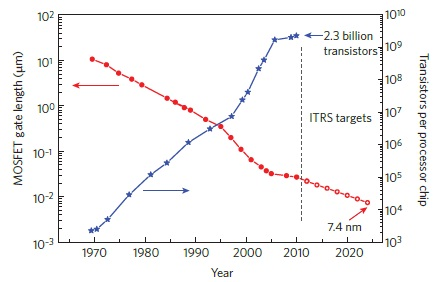
\includegraphics[width=9cm, height=5cm]{2.jpg}
\caption{Evolution of MOSFET gate length shown with (red circle). As gate lengths have decreased, the number of transistors per processor chip has increased (blue stars).}
\end{figure}

This paper is organized as follow: Section-I gives the Introduction about Graphene based semiconductor technology. Section-II will give the insight to understand the nature and properties of graphene. Section-III talks about the possibilty of making electronics devices such as transistors using graphene based nanotechnology. Section-IV shows some special properties that graphene transistors have. Section-V talks about the future scope of the graphene based nanotechnology and at the end Section-VI concludes paper and followed by references.

\section{\textbf{The Origin of Graphene}}
Graphene is made by bounding the carbon atom together in a network of hexagons repeating itself within a single plane which has a thickness of one atom. It is excellent conductor of heat, electricity, energy and since carbon is all around us which makes it a common element, makes it a vialable and excellent choice for creating cheaper integrated circuits. The electron mobility of graphene is above 15000 $cm^2$/VS but theoretical limits is 200000 $cm^2$/VS at room temperature which is about “30 times GaAs, 100 times that of Silicon, and even larger than carbon nanotubes". It is only material in electronics we have known in which electrons at room temperature can move about thousands of interatomic distance without getting scattered all around in the bulk of the material.

\begin{figure}[h]
\centering
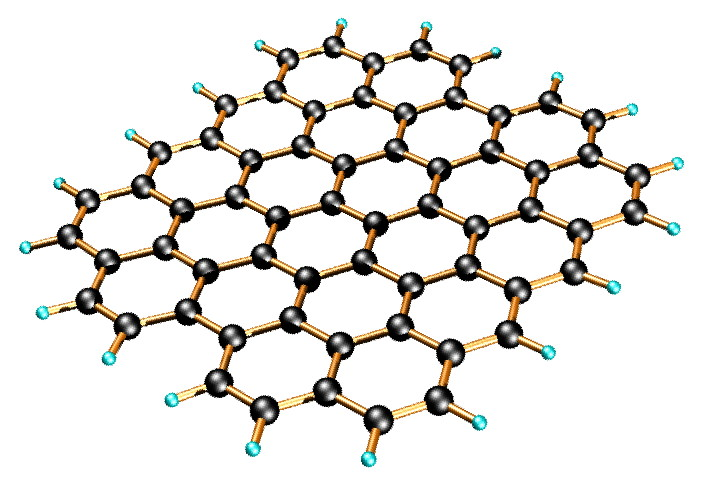
\includegraphics[width=5cm, height=3.2cm]{graphene.jpg}
\caption{Graphene is an atomic-scale honeycomb lattice made of carbon atoms.}
\end{figure}

\subsection{\textbf{Graphene Structure}}
Graphene, is a single atom thick sheet of carbon atoms. It is an allotrope of carbon that is made up of tightly bonded carbon atoms aligned together into a hexagonal space lattice. Graphene has $sp^2$ hybridisation and has a interatomic thickness of about 0.345nm. These properties enable graphene to break so many limits that traditional material are not capable of such as very high mechanical strength, very high conductivity etc. Now we must look into the intrinsic properties which separate it from other allotrope of carbons and other materials.

\subsection{\textbf{Fundamental Properties of Graphene}}
In the year 2004 researchers have isolated monolayer Graphene, and they thought that theoretically 2-D compounds could not exist due to thermal instability. However, some researchers managed to isolate graphene and showed the world that it is possible to actually isolate and produce graphene, but it took some time for the researchers to do so. Researchers at that time studied electron transmission using electron microscopy, after that they slightly modified the structure of the material. However, later researches found out the fact that the carbon to carbon bonds in graphene are so small and strong that they prevent thermal fluctuations from de-stabilizing the material.

\subsubsection{\textbf{Electronic Properties}}
Graphene is only material known to us which has no ``Band Gap", it is a semi-metal with both holes and electrons as charge carries. It has very high electrical conductivity. Carbon atoms have a total of 6 electrons, 4 in the outer shell and 2 in the inner shell. The 4 electrons in the outer shell are responsible for chemical bonding with the neighbouring carbon atoms, but in case of Graphene, each atom is bonded with 3 other carbon atoms in a 2-D plane, therefore leaving 1 electron free. This freely available electron in responsible for high electrical conductivity. These highly mobile eletrons are called pi-elctrons and are located above and below the graphene sheet. Due to these pi orbitals overlap and enhances the carbon to carbon bonds in graphene, therefore appealing towards more thermal stability of graphene.
\\

\subsubsection{\textbf{Mechanical Strength}}
Another of graphene’s stand-out properties is its unbeatable meachanical strength. Graphene is the strongest material ever discovered, with an unbelievable tensile strength of 130 Gigapascals. With it's extraodinary mechanical strength, it is also very light weight about 0.77 mg per $m^2$. Graphene also contains elastic properties, and it is able to retain it's intial shape after hard strain, this is a particularly special properties of graphene but their a glitch, it is very difficult and costly to produce graphene that is containing no imperfections i.e. unflawed. But production technique are evovling with time and they are being designed with an ultimate goal of reducing the cost and complexity for producing graphene.

\subsection{\textbf{Graphene Properties Relevant To Electronics}}
In this section, I discuss two important aspects of graphene: the concept of bandgap in graphene, and charge transport phenomena at room temperature.

\subsubsection{\textbf{Band Gap}}
We know that graphene is a semi-metal with zero bandgap. It's conduction bands and valence bands are of conical shape and they meet at the K points of the Brillouin zone. Because the bandgap is zero in graphene, we are facing a problem, we cannot make devices for digital logic applications because we cannot control switching of the device. However, researchers and scienctists have found out a way to control the band strucuture of graphene by modifiying it's band structure. It can be done in 3 ways: by biasing bilayer graphene, by constraining large-area graphene in one dimension and by applying strain to graphene.
\\
\begin{figure}[h]
\centering
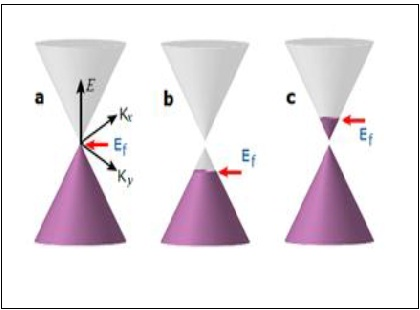
\includegraphics[width=7cm, height=4.2cm]{1.jpg}
\caption{Schematic band structures of graphene. (a) Band structure of graphene with zero-bandgap. Ef is at the cross-over point. Band tructures of (b) p-type and (c) n-type graphene with the bandgap. Ef lies in valence and conduction band, respectively.}
\end{figure}

\subsubsection{\textbf{Carrier Mobility}}
The most usable and valuable advantage of using graphene is that, it has very high carrier mobility at room temperature. The range of mobility is between 10000 - 15000 $cm^2$/VS for graphene with an upper limit between 40000 - 70000 $cm^2$/VS. Moreover, in the absence of charged impurities, mobilities of around 200000 $cm^2$/VS have been predicted. The graphene having a large area which is grown on nickel in labs and then transferred to a substrate, found with mobilities greater than 3700 $cm^2$/VS.
\\

During the early production stages of MOSFET using graphene, researchers found out that the mobility was affected by the material used for making the top-gate dielectric for the MOSFET. However, in the recent times researchers found out that high-mobility graphene MOS channels can be made with the proper choice of the material used for making the dielectric for the top-gate for the MOSFET and optimized doping process.
\\

\section{\textbf{Era Of Graphene Transistors}}
With the evolution of transistor semiconductor technology, researchers and scienctist all around the world have work together and they have developed the method to carve graphene into tiny electronics circuits with transistors having a size comparable to that of a molecule. Their is a say from researchers at manchaster that ``The smaller the size of the transistors the better is their performance".
In the last few years, the researchers at manchaster broke the record by making the smallest transistor using graphene.
\\

It has been found out that transistor made from graphene flakes form lumps of graphite and get stuck to the substrate and they assure highest performance than the transistor which are made on graphene formed on the surface of substrates. Here we will talk about the two outstanding technique used by the manufacturers in order to produce transistor based on graphene nanotechnology:
\\

\subsection{\textbf{Production Method:}}
\subsubsection{\textbf{First Production Method}}
In the last few years, manufacturers used to make transistor using graphene by placing a sheet of graphene on the top of an insulating substrate, such as SiO$_2$. However, as we have talked earlier about the substrate choice, we know the this substrate can degrade the electronic properties of the transistor. However, scienctist have found out a solution to this problem, and figure it out that, using a diamond like carbon placed on the top layer of the substrate of a wafer of silicon, due to nonpolar nature of carbon, it does not scatter charges as SiO$_2$ does alone. Experimentally it was found out that this new transistor is much more stable in temperature ranging from extreme cold like that in space and hot as that of near boiling water. It was found out during experimentation that this device can operate upto speed of 155GHz(extremely fast) with low power consumption. These new high frequency devices have applications in communications.
\\

\subsubsection{\textbf{Second Production Method:}}
In this method, what researchers do is that, they have made transistors using graphene grow directly on substrate which is insulated with a promient structure. In this process, we start by taking a iron film catalyst over an oxide film on a Si substrate.

\begin{figure}[h]
\centering
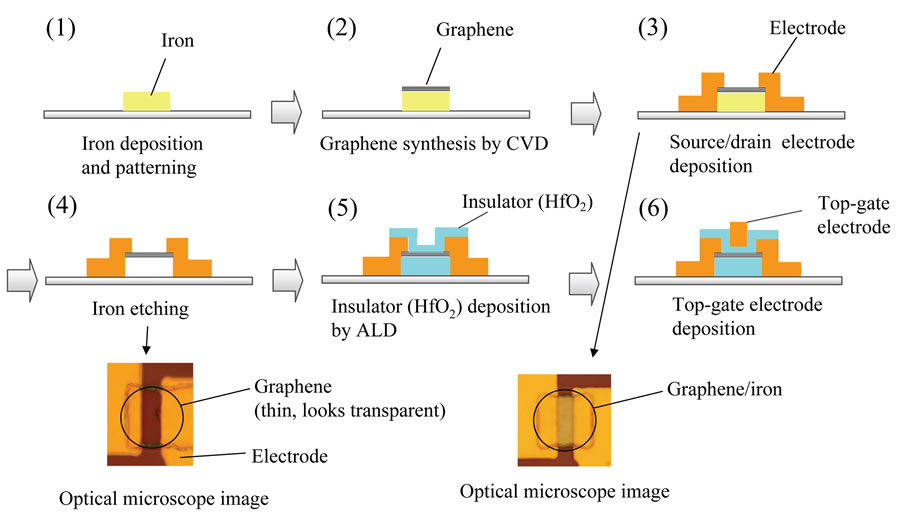
\includegraphics[width=9cm, height=7cm]{3.jpg}
\caption{Industrial Process For Making Transistor Using Graphene}
\end{figure}

The process to make transistors is, the iron bars used above is first converted into strips using a technique called photolithography before graphene is grown on the bars. As soon as the graphene is grown on the bars, source and drain electrodes are formed at the ends of each graphene strip using titanium gold film. With this done, we will see that this will leave the centre, which will become the channel, when exposed. We have seen that the source and drain are bonded at ends of the graphene strip to the substrate, this allows the iron bar under it to be etched away with use of the acid inorder to make a graphene channel suspended as a bridge for electrons. We use HfO$_2$ as insulator, HfO$_2$ is grown on the top of the channel to form an insulation for the gate which is going to laid down on the top. This method enables manufacturer to form graphene transistor across the entire surface of the substrate. As graphene semiconductor technology in only about a few nanometer thick, it is perfect candidate for use in material making up for thin-film transistor used in video displays.
\\

We can maufacture these new graphene transistor by utilizing the technologies which are already being developed for standard silicon based semiconductor technology. We just need to slightly modify these techniques for production of Graphene based semicondutor technology.
\\

\subsection{\textbf{Graphene Field Effect Transistors(GFETs):}}
The most straightforward device application of graphene semiconductor technology is making channel MOSFETs in replacement of those Si based MOSFETs. Fig. 5a). shows the schematic of graphene field effect transistor, including gate dielectric and source and drain metal contacts and a top gate electrode. Fig. 5b). shows the top-view of the optical micrograph of a macroscopic graphene field effect transistor on SiO$_2$.

\begin{figure}[h]
\centering
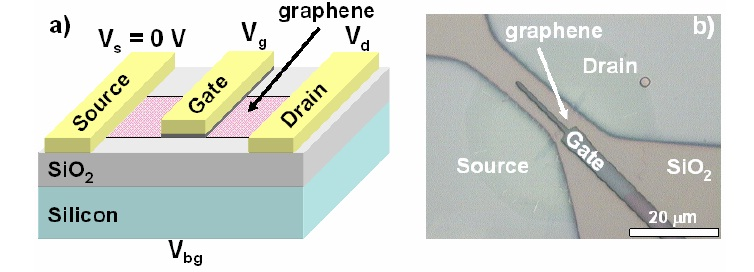
\includegraphics[width=9cm, height=5cm]{4.jpg}
\caption{a).Schematic cross section area and b).Optical top-view micrograph of a graphene field effect transistor}
\end{figure}

The fabrication process of graphene FETs is pretty tedious, it follows the standard Si process technology. Here once the graphene is identified and deposited, use of techniques called photo-lithography, reactive ion etching and thin-film deposition for the gate insulators and contacts takes place. Here, in Fig. 6a).The tranfer characterstics (drain current Id vs back gate voltage Vbg) of graphene transistor. Here from the figure we observe a major drawback of GFETs; The absence of band gap (Eg = 0eV) atonishingly affect the current modulation in the GFETs and lead to ambipolar behavior. In fact, the best current modulation reported to date is about 30, which were measured at very low cryogenic temperatures. 

\begin{figure}[h]
\centering
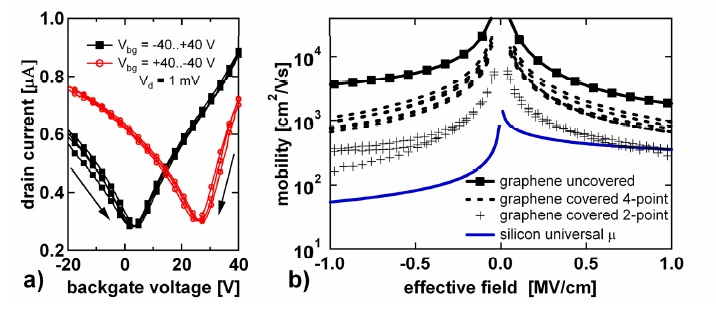
\includegraphics[width=9.35cm, height=5.5cm]{5.jpg}
\caption{a).Drain current versus back gate voltage of a graphene FET. b).Mobility versus electric field in graphene FET.}
\end{figure}

Futhermore, it has been found out through experimentation that the zero band gap leads to finite amount of charge density without applying any gate voltage and it is also verified the GFETs conduct substantial amounts of current at their point of minimum conducatance, therefore this prevents the application of GFETs in CMOS logic circuitry.
\\

When Graphene suspended measured in very high vacumm conditions has shown mobilities exceeding 200000 $Cm^2$/VS, but in real scenrios the GFETs performance is limited by choice of substrates and top gates. But this doesn't mean that GFETs have no application in real life, the carrier mobility in top-gate device made from graphene exceed those of Si and are typically inorder pf several of thousand $Cm^2$/VS. 
\\

\section{\textbf{Some Special Properties of Graphene Transitors}}
Graphene has got a lot of interesting properties but here we will just consider only two of these properties.
\\

\subsection{\textbf{Self-Cooling GFETs:}}
The one thing that disturbs an electronics engineer the most is the energy lost in the form of heat. Heat is the sad fact of the electronic devices we use. Each and every device generates heat which affect it's functioning some way or the other. By today's standard, a temperature of about 75 degrees is a minimal temperature at which mordern CPUs and GPUs works, so it is a pretty high temperature at which our todays mordern circuitry works. But that could all soon change. While examining transistors made from graphene, researchers noticed that they have ability to ``SELF-COOL". Because of the extremely thin size of graphene transistor, it is very difficult to measure accurately the certain parameters of the material.
\\

It was observed during the experimentation that resistive heating effect in graphene was weaker than its themo-electric cooling effect.
In Si and most of the other material used for making electronic devices, the electronic heating effect is much dominant than self-cooling. However, through more expermentation it has been found out that their are regions where thermo-electric cooling is much larger than resistive heating. This means that graphene circuitry does not heat up like it traditional Si based circuitry. This means and motivates us to use graphene circuitry in our day to day life.
\\

\subsection{\textbf{Low Noise Generation Capability:}}
For any electronics to be useful in analog and digital circuitry, the level of the electronic low frequency noise has to be decreased to a certain acceptable level. The noise spectrum is dominated by the low frequency electronic noise upto 100Khz. Researchers all around the world our trying to fabricate graphene transistor with very low frequency noise. They are developing new fabrication technique in order to achieve the above goal of low noise generation. The low frequency noise in the traditonally used transistor is characterized by a parameter known as Hooge parameter. In traditonal materials, the Hooge parameter is of the order of $10^-$$^5$ to $10^-$$^3$. In graphene based semiconductor technology, the Hooge parameter is of order $10^-$$^4$ to $10^-$$^2$. From further experimentation researchers found out that low frequency noise generation is dominated by the fluctuations in the carrier density due to trapping and de-trapping by the defects(specific energy levels). This means that we can even further reduce the noise level by upgrading our fabrication techniques.
\\

\section{\textbf{Future of Graphene Semiconductor Technology}}
As we have seen in the present time that this 2-D material, Graphene, has shown promising capabilities to make electronics smaller and more efficient. In the near future, researchers are trying to build graphene-based transistor that works with ultra-low power and with clock speed up to a staggering 100 GHz. Scientist and researchers are working in small group together inorder to acheive very high speed and low power consumptions graphene based transistor, they are analysing the properties of the graphene, mixing and fusing them with other material to make transistor more controllable. They are trying to stablize the quantum tunneling effect and when this is done they will get the same functionality as that of Si based transistor with much lower voltage applied onto the gate and higher efficiency and switching speeds, therefore ``Chips will require less power to operate, less heat will be produced, less poweful cooling engines will be needed, and overclocking can be done easily without any worry that the excess heat will destroy the chip"
\\

As the graphene semiconductor technology evovles, we will have devices which consumes very less power and can now run for days instead of hours, we will see computing power which was not even thought of, we will be able to perform complex calculations very easily within a small span of time. We will become the witness how the world around us changes, as the semiconductor technology is the heart and soul of all the electronics we see around us, if this changes, then all the things around us changes. We will see how the bilayer graphene technology will change the world, it will be the first step towards drastically increased computing power. We can now dream of computing power with not 1GHz not even 10GHz, may be astonishing 100GHz.
\\

\section{\textbf{Conclusion}}
I would conclude this paper by saying that, their is a tremendous potential hidden in the 2-D single atom thick sheet of carbon, Graphene, the devices made using this semiconductor technology have grown in the past few years, and they will become the best of choice and will eventually replace Si based semiconductor devices completely. This paper was all about to show researchers and other people that graphene has a tremendous potential hidden in it, these types of demonstrations are important because graphene has the capability to the push the limits of Si based semiconductor technology and infact it is pushing the limits. It properties may not be ideal, but they are impressive. Their are many advantages of using graphene transistor technology, its high carrier mobility makes it perfect for high speed applications, having ideal electrostatic behaviour enables aggressive scaling, and direct integration with present CMOS technology. But their is dark side to graphene also, graphene has a zero energy band gap, so this means that it will conduct a lot of electrons even when it is switched off, that would count for a large amount of energy getting wasted but these problems can be solved and parameters of the devices can be improved with better fabrication techniques.
\\ \\

\begin{thebibliography}{6}

\bibitem{Bhupendra}
\textbf{Bhupendra K. Sharma, Jong-Hyun Ahn}: Graphene based field effect transistors: Efforts made towards flexible electronics,
\\\textit{http://www.sciencedirect.com/science/article/pii/S0038110113002803}\\

\bibitem{Frank}
\textbf{Frank schwierz}: Graphene transistors,
\\\textit{http://www.nature.com/nnano/journal/v5/n7/full/nnano.2010.89.html}\\

\bibitem{T}
\textbf{T. Ihn, J. Güttinger, F. Molitor, S. Schnez, E. Schurtenberger, A. Jacobsen, S. Hellmüller, T. Frey, S. Dröscher, C.Stampfer, K. Ensslin}: Graphene single electron transistors,
\\\textit{https://www.nano.phys.ethz.ch/~ihn/papers/IhnGraphene10.pdf}\\

\bibitem{Alexander}
\textbf{Alexander V. Klekachev, Amirhasan Nourbakhsh, Inge Asselberghs, Andre L. Stesmans, Marc M. Heyns, and Stefan De Gendt}: Graphene Transistors and Photodetectors,
\\\textit{https://www.nano.phys.ethz.ch/~ihn/papers/IhnGraphene10.pdf}\\

\bibitem{Johanna}
\textbf{Johanna Anteroinen}: Graphene transistors challenges and opportunities,
\\\textit{https://wiki.aalto.fi/download/attachments/107190425/Johannanlisuri.pdf}\\

\bibitem{Nanowerk}
\textbf{Nanowerk Publications}: Graphene transistors can work without much noise,
\\\textit{http://www.nanowerk.com/spotlight/spotid=11630.php}

\end{thebibliography}

\end{document}
